%%%%%%%%%%%%%%%%%%%%%%%%%%%%%%%%%%%%%%%%%%%%%%%%%%%%%%%%%%%%%%%%%%%%%%%%%%%%%%%
% Chapter 4: Tecnologías
%%%%%%%%%%%%%%%%%%%%%%%%%%%%%%%%%%%%%%%%%%%%%%%%%%%%%%%%%%%%%%%%%%%%%%%%%%%%%%%

Uno de los puntos más importantes de este trabajo era determinar las diferentes tecnologías
a utilizar. El mundo web ha sufrido una gran revolución en los últimos años y ahora
se disfruta de una gran variedad de propuestas para cada tipo de tarea.

Es por ello, que ha habido que hacer una gran valoración del estado del arte 
tecnológico para determinar qué curso debería seguir la aplicación.

%++++++++++++++++++++++++++++++++++++++++++++++++++++++++++++++++++++++++++++++
\section{Lenguaje para la lógica de la aplicación}
\label{4:sec1}
Por normal general cuando se habla de programación web en el lado del cliente, se tiende a pensar
de forma inmediata en Javascript, y en general, este razonamiento es indudablemente válido. 
Pero dado que SIMDE es una aplicación fuertemente orientada a objetos y con una gran base de código, 
se han valorado múltiples alternativas con el objetivo de agilizar la realización de este proyecto.

\subsection{Coffescript}

Coffescript es un pequeño lenguaje que se compila en Javascript, su objetivo era mejorar la legibilidad 
y concisión de Javascript añadiendo varios \textit{syntactic sugars} inspirados en otros lenguajes como
\textit{Ruby} o \textit{Python}. \cite{Coffescript}

\bigskip
Coffescript es un lenguaje con un largo recorrido, apareciendo a finales del año 2009. Y tiene soporte por
parte de \textit{Ruby on Rails} y \textit{Play framework}. \cite{CoffescriptWiki}

\bigskip 
Coffescript podría ser la opción ideal para agilizar le desarrollo debido a la similitud de sintaxis con 
Ruby.

\begin{lstlisting}
class Animal
  constructor: (@name) ->

  alive: ->
    false

class Parrot extends Animal
  constructor: ->
    super("Parrot")

  dead: ->
    not @alive()
\end{lstlisting}

\bigskip
Sin embargo, la opción de Coffescript ha sido desestimada en gran medida por su decreciente popularidad
y la poca certeza del futuro que tomará el lenguaje.

\subsection{Dart}

Dart es un lenguaje de código abierto desarrollado por Google que permite desarrollador aplicaciones web, móvil, 
de servidor y también se puede utilizar en el \textit{Internet of Things}. \cite{Dart}

\bigskip
Se ha considerado en el desarrollo de esta aplicación porque es un lenguaje orientado a objetos que utiliza una 
sintaxis similar a C\#. Además, aunque Google Chrome tiene una máquina virtual nativa para este lenguaje, es posible
transpilar el código a Javascript para los navegadores que no tiene este soporte nativo.

\bigskip
Tras razonar detenidamente, ha pesar de lo atractivo del lenguaje, Dart ha quedado descartado por 
una razón de peso y es que se trata de un lenguaje totalmente diferente y su uso es mayoritariamente
por parte de Google.

\subsection{Typescript}

Typescript es un lenguaje libre y de código abierto desarrollado por Microsoft que actúa como un superconjunto
de Javascript, es decir incorpora los distintos estándares: ECMA5, ECMA6, ECMA7... Y además, como característica
destacable, añade comprobación de tipos en tiempo de compilación. \cite{Typescript}

\bigskip
Este tipado no se refleja en el código final, de hecho una interfaz, por ejemplo,
añade 0 sobrecarga en el código final. Pero si que es interesante por las capacidades de
autocompletado (a través de Microsoft Intellisense)  que añade.

\begin{figure}[!th]
\begin{center}
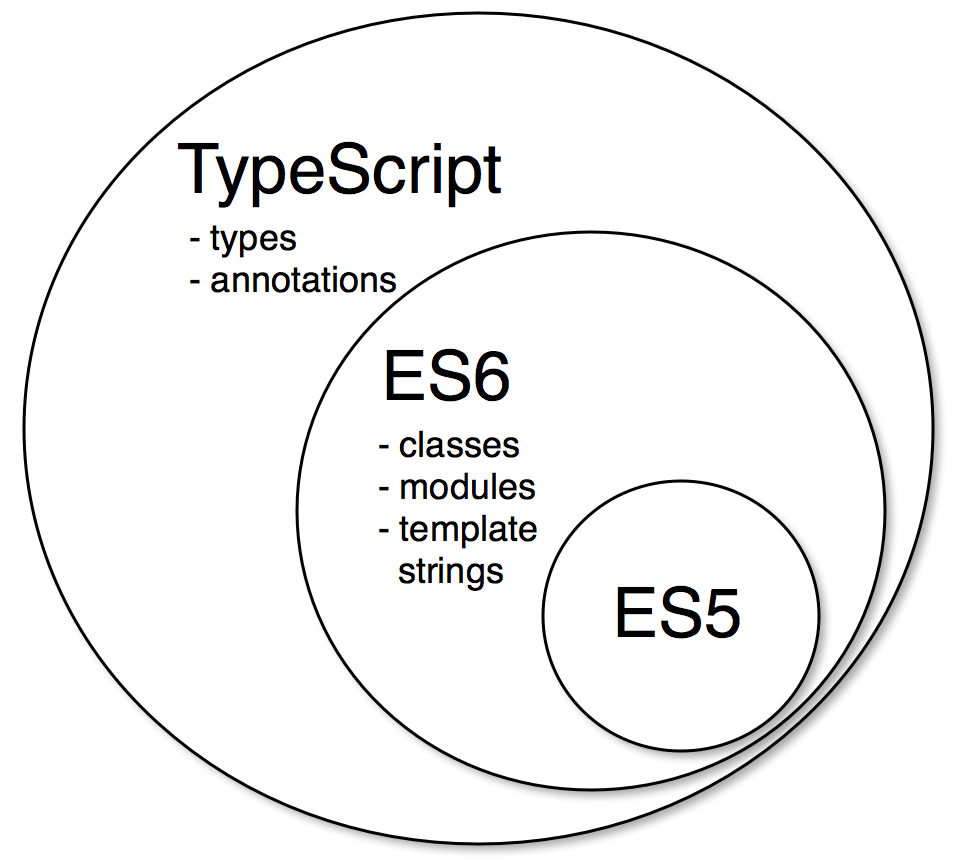
\includegraphics[width=0.5\textwidth]{images/cap4/typescript.eps}
\caption{Typescript como superconjunto de Javascript}
\label{fig:Typescript como superconjunto de Javascript}
\end{center}
\end{figure}

\bigskip
Al final, en este proyecto Typescript ha sido la tecnología ganadora, y existen múltiples
razones:

\begin{enumerate}

\item Typescript tiene bastante apoyo por parte de la comunidad y por parte de la propia Microsoft.
La documentación es extensa y efectiva.

\item Typescript está alineada en cierta forma con el futuro de Javascript. Microsoft es uno de los 
muchos que forman parate del concenso de estándar de ECMASCRIPT.

\item Typescript no me limita en la posibilidad de usar javascript, todo código javascript es código
Typescript válido.

\item Por último y no menos importante: Tengo cierta experiencia con Typescript.
\end{enumerate}



%++++++++++++++++++++++++++++++++++++++++++++++++++++++++++++++++++++++++++++++
\section{Tecnología para la integración modelo vista}
\label{4:sec2}
Desde el inicio del proyecto, se tenía claro que alguna librería se encargaría de gestionar
 el tedioso proceso de manipular el DOM. Actualmente existen múltiples librerías 
y frameworks que podían servir para realizar esta tarea, pero muchos de ellos (como por ejemplo Angular),
son demasiado \textit{rígidos} y acaban condicionando la forma de desarrollar la aplicación, 
lo cual resulta ser contraproducente.

\subsection{Webcomponents}

\bigskip
Una de las características más deseadas para el nuevo diseño de la interfaz de SIMDE era contar con
un diseño basado en componentes. Siendo la caracteŕistica más deseada de todo el incorporar las nuevas 
ventajas que ofrecen los \textit\textbf{Web Components}. Los Web Components son un conjunto de 
características que se están añadiendo a las especificaciones W3C de Html y del DOM. \cite{Webcomponents}

\bigskip 
El objetivo de estas características es permitir crear componentes personalizados, reusables y 
con su propia encapsulación. Esto se consigue a través de cuatro características principales:

\begin{enumerate}

\item \textbf{Elementos personalizados}: Esta característica permite diseñar y utilizar nuevos tipos 
de elementos del DOM.
\item \textbf{Shadow DOM}: Esta característica permite al navegador incluir un subarbol de elementos del 
DOM en el renderizado del documento pero \textbf{NO} se incluyen el DOM principal.
\item \textbf{HTML Imports}: Esta característica permite incluir y reutilizar documentos HTML en otros 
documentos HTML.
\item \textbf{Plantillas HTML}: Esta característica permite declarar fragmentos de código de marcas que no
se utilizan en el carga de la página pero que se pueden instanciar en tiempo de ejecución. 

\end{enumerate}

\subsection{Polymer}
Esta librería fue la primera que hizo uso de los Web Components.Desarrollada por Google y anunciada en 
el año 2013, Polymer permite aprovechar las características de los Web Components \cite{Polymer} a través de los polyfills 
-códigos que implementan características en los navegadores que no soportan las mismas de forma nativa-.
\textit{(Comúnmente se conoce como polyfill a la librería que implementa el estándar de HTML5)}. \cite{Polyfill} 

\bigskip
A pesar de la revolución que marcó, Polymer no fue ampliamente acogida por la comunidad de desarrolladores 
-quizás por ser una librería adelantada a su tiempo-. Y hoy en día nos encontramos con otro intento por 
parte de ganar peso en la comunidad: Polymer 2.0. Esta nueva versión incorpora el soporte de las clases de ES6
y además permite utilizar el método de la especificación de custom elements v1 para definir elementos.

\bigskip
Aunque las mejoras que incorpora Polymer 2.0 la hacen una opción totalmente válida y viable, aún no 
tiene una comunidad lo suficientemente sólida con lo que esto acaba traduciéndose en una menor 
cantidad de recursos disponibles.

\subsection{React}
La empresa autora de esta librería de código abierto, Facebook, la define como: “It’s a Javascript library for building UI’s”. \cite{React}

\bigskip
Pero realmente aunque esta declaración es totalmente cierta, React no es tan algo tan simple. Para resolver el problema
 de la modificación del DOM de una forma eficiente: Simulándolo esta estructura en memoria y aplicando diversos
 algoritmos para calcular cuales serían los mínimos cambios necesarios a realizar sobre el \textit{DOM verdadero}
 para representar los diversos cambios de estado.

\bigskip
React se basa en el uso de componentes, no en el sentido explícito de los \textit{Web Components} tal como los define 
el éstandar de HTML5, sino como pequeños bloques reusables que incorporan cierta funcionalidad. Sin embargo, a pesar 
de que React se puede integrar con la api de \textit{Web Components}, el uso de esta api incrementa de forma exponencial
la complejidad de la aplicación, con lo cual se ha pospuesto el uso de esta característica para versiones futuras.


\bigskip
React utiliza un híbrido entre html y javascript denominado jsx, como también tiene soporte para 
Typescript, en este caso utilizamos tsx.

\begin{figure}[!th]
\begin{center}
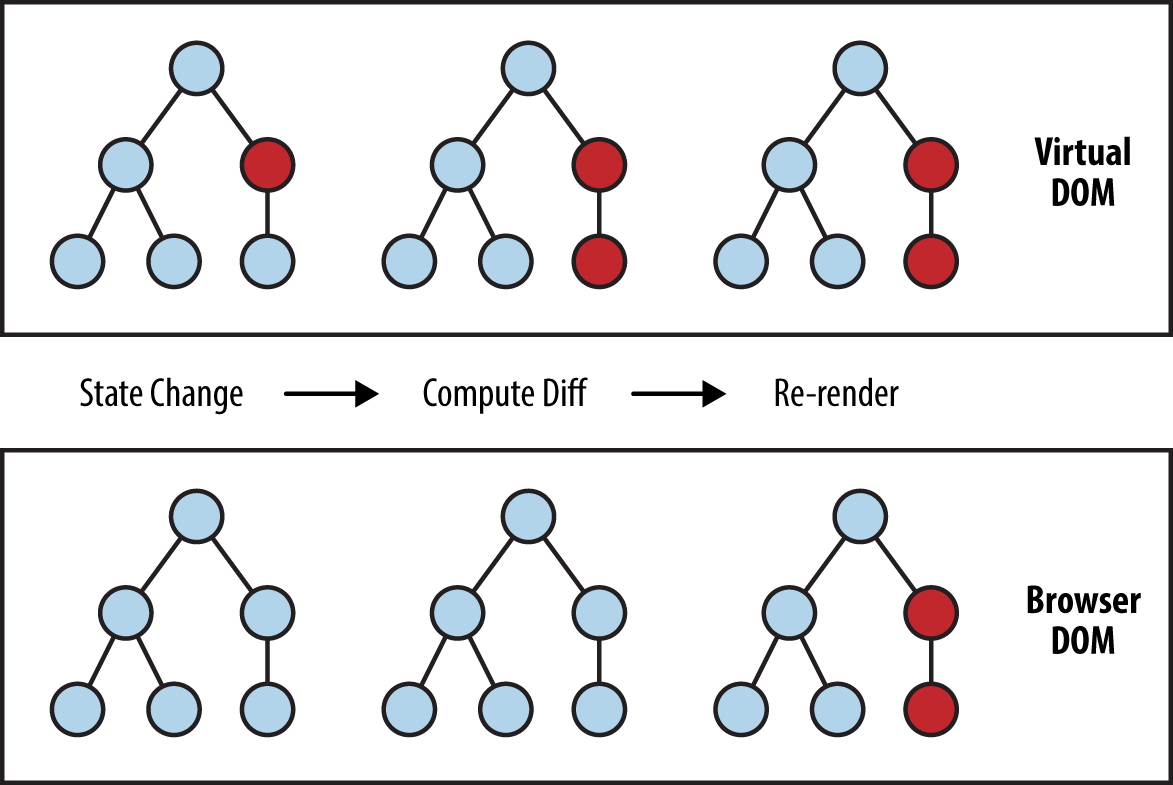
\includegraphics[width=0.8\textwidth]{images/cap4/react-virtual-dom.eps}
\caption{Funcionamiento del DOM virtual de React \cite{ReactVirtualDOM}}
\label{fig:Funcionamiento del DOM virtual de React}
\end{center}
\end{figure}

\bigskip
React es ampliamente utilizada por muchísimas empresas gracias a su capacidad de integrarse con otras librerías. 
Por ejemplo Microsoft mantuvo parte de la página en jQuery mientras iba integrando React.

\bigskip
Otro ejemplo de grandes empresas que hagan uso de esta librería son: AirBnB, Netflix, Wallmart…  \cite{ReactUsers}

\bigskip
Y muchas de ellas han contribuido al ecosistema de React, ya sea mediante guías de estilo, conjunto de componentes, patrones... \cite{ReactStyleGuide}

\bigskip
Además,la comunidad de usuarios es increíblemente activa, por ejemplo es común ver a Dan Abramov resolviendo dudas
en distintos sitios como \textit{Github} o \textit{Reddit}. Dan Abramov es el creador de Redux (una implementación de gestión de estados), desarrollador de la nueva implementación de 
React \textit{(react-fiber)}, empleado de Facebook, participante en muchas conferencias y además autor de 
múltiples herramientas como \textit{react-hot-loader}. 

\bigskip
Debido a todo lo anterior y a que además, React tiene una excelente integración con Typescript utilizando 
el formato .tsx, queda claro que es la mejor opción posible para esta aplicación. React es una librería 
desarrollada por Facebook para construir interfaces.


%++++++++++++++++++++++++++++++++++++++++++++++++++++++++++++++++++++++++++++++
\section{Tecnología para hacer la build}
\label{4:sec3}
Debido a la complejidad de las aplicaciones web modernas, es necesario 
realizar una serie de pasos intermedios entre el código original y 
el resultado final de la apliación. Para el caso de este proyecto, se debe:

\begin{itemize}

\item Compilar el código typescript a javascript.

\item Compilar el código .tsx a .jsx.

\item Resolver las importaciones de dependencias, tanto de la lógica
como de los componentes.

\item Procesar el código sass y convertirlo en css.

\end{itemize}

\subsection{Gulp/Grunt}

La primera tendencia -debido a su gran extensión- sería utilizar 
lo que se conoce como un \textit{task runner}. Actualmente, dos de los 
más conocidos son \textbf{Grunt} \cite{grunt} y  \textbf{Gulp} \cite{gulp}.

\bigskip
Ambos están basados en NodeJs y son compatibles entre sí en gran medida.
Su funcionamiento es sencillo, en un gruntfile o gulpfile se definen las tareas a
ejecutar, seleccionando los ficheros de fuente sobre los que actuar -si cabe- y la tarea 
a realizar.

\bigskip
Existen muchisimos plugins desarrollados que permiten hacer todo tipo de tareas, desde traducir
markdown hasta minimizar el contenido de los ficheros de estilos y de javascript.

\bigskip
Sin embargo, a pesar de que esta opción era altamente atractiva debido 
a su robustez, se ha optado por probar una solución aún más moderna, \textbf{webpack}.

\subsection{Webpack}

Webpack es un \textit{empaquetador de módulos} para aplicaciones de Javascript modernas.
Cuando webpack procesa la aplicación, construye un grafo de dependencias
incluyendo todos los módulos y luego lo empaqueta en orden \cite{webpack}.  

\bigskip
Webpack incorpora de serie diversas características interesantes tales como el 
poder ejecutar un servidor de desarrollo que aplica \textit{hot reloading} sobre el código 
sin requerir refrescar la página o el poder separar el código css/js de terceros para el 
entorno de producción. 

\bigskip 
El funcionamiento de webpack puede ser extremadamente resumido y simplificado en:

\begin{itemize}

\item Partiendo de un punto de entrada, una serie de reglas sobre los distintos tipos de ficheros
activan una serie de \textit{loaders} correspondientes para procesarlos. 

\item Estos loaders pueden ser concatenados entre sí para obtener el resultado deseado, por ejemplo
podemos traducir el código typescript a es6 para luego traducir este código junto a otro a es5 mediante
babel.

\item Se aplican, si fuera necesario, el uso de plugins para tareas más complejas que se quieren aplicar sobre
todos los paquetes.

\end{itemize}

\begin{figure}[!th]
\begin{center}
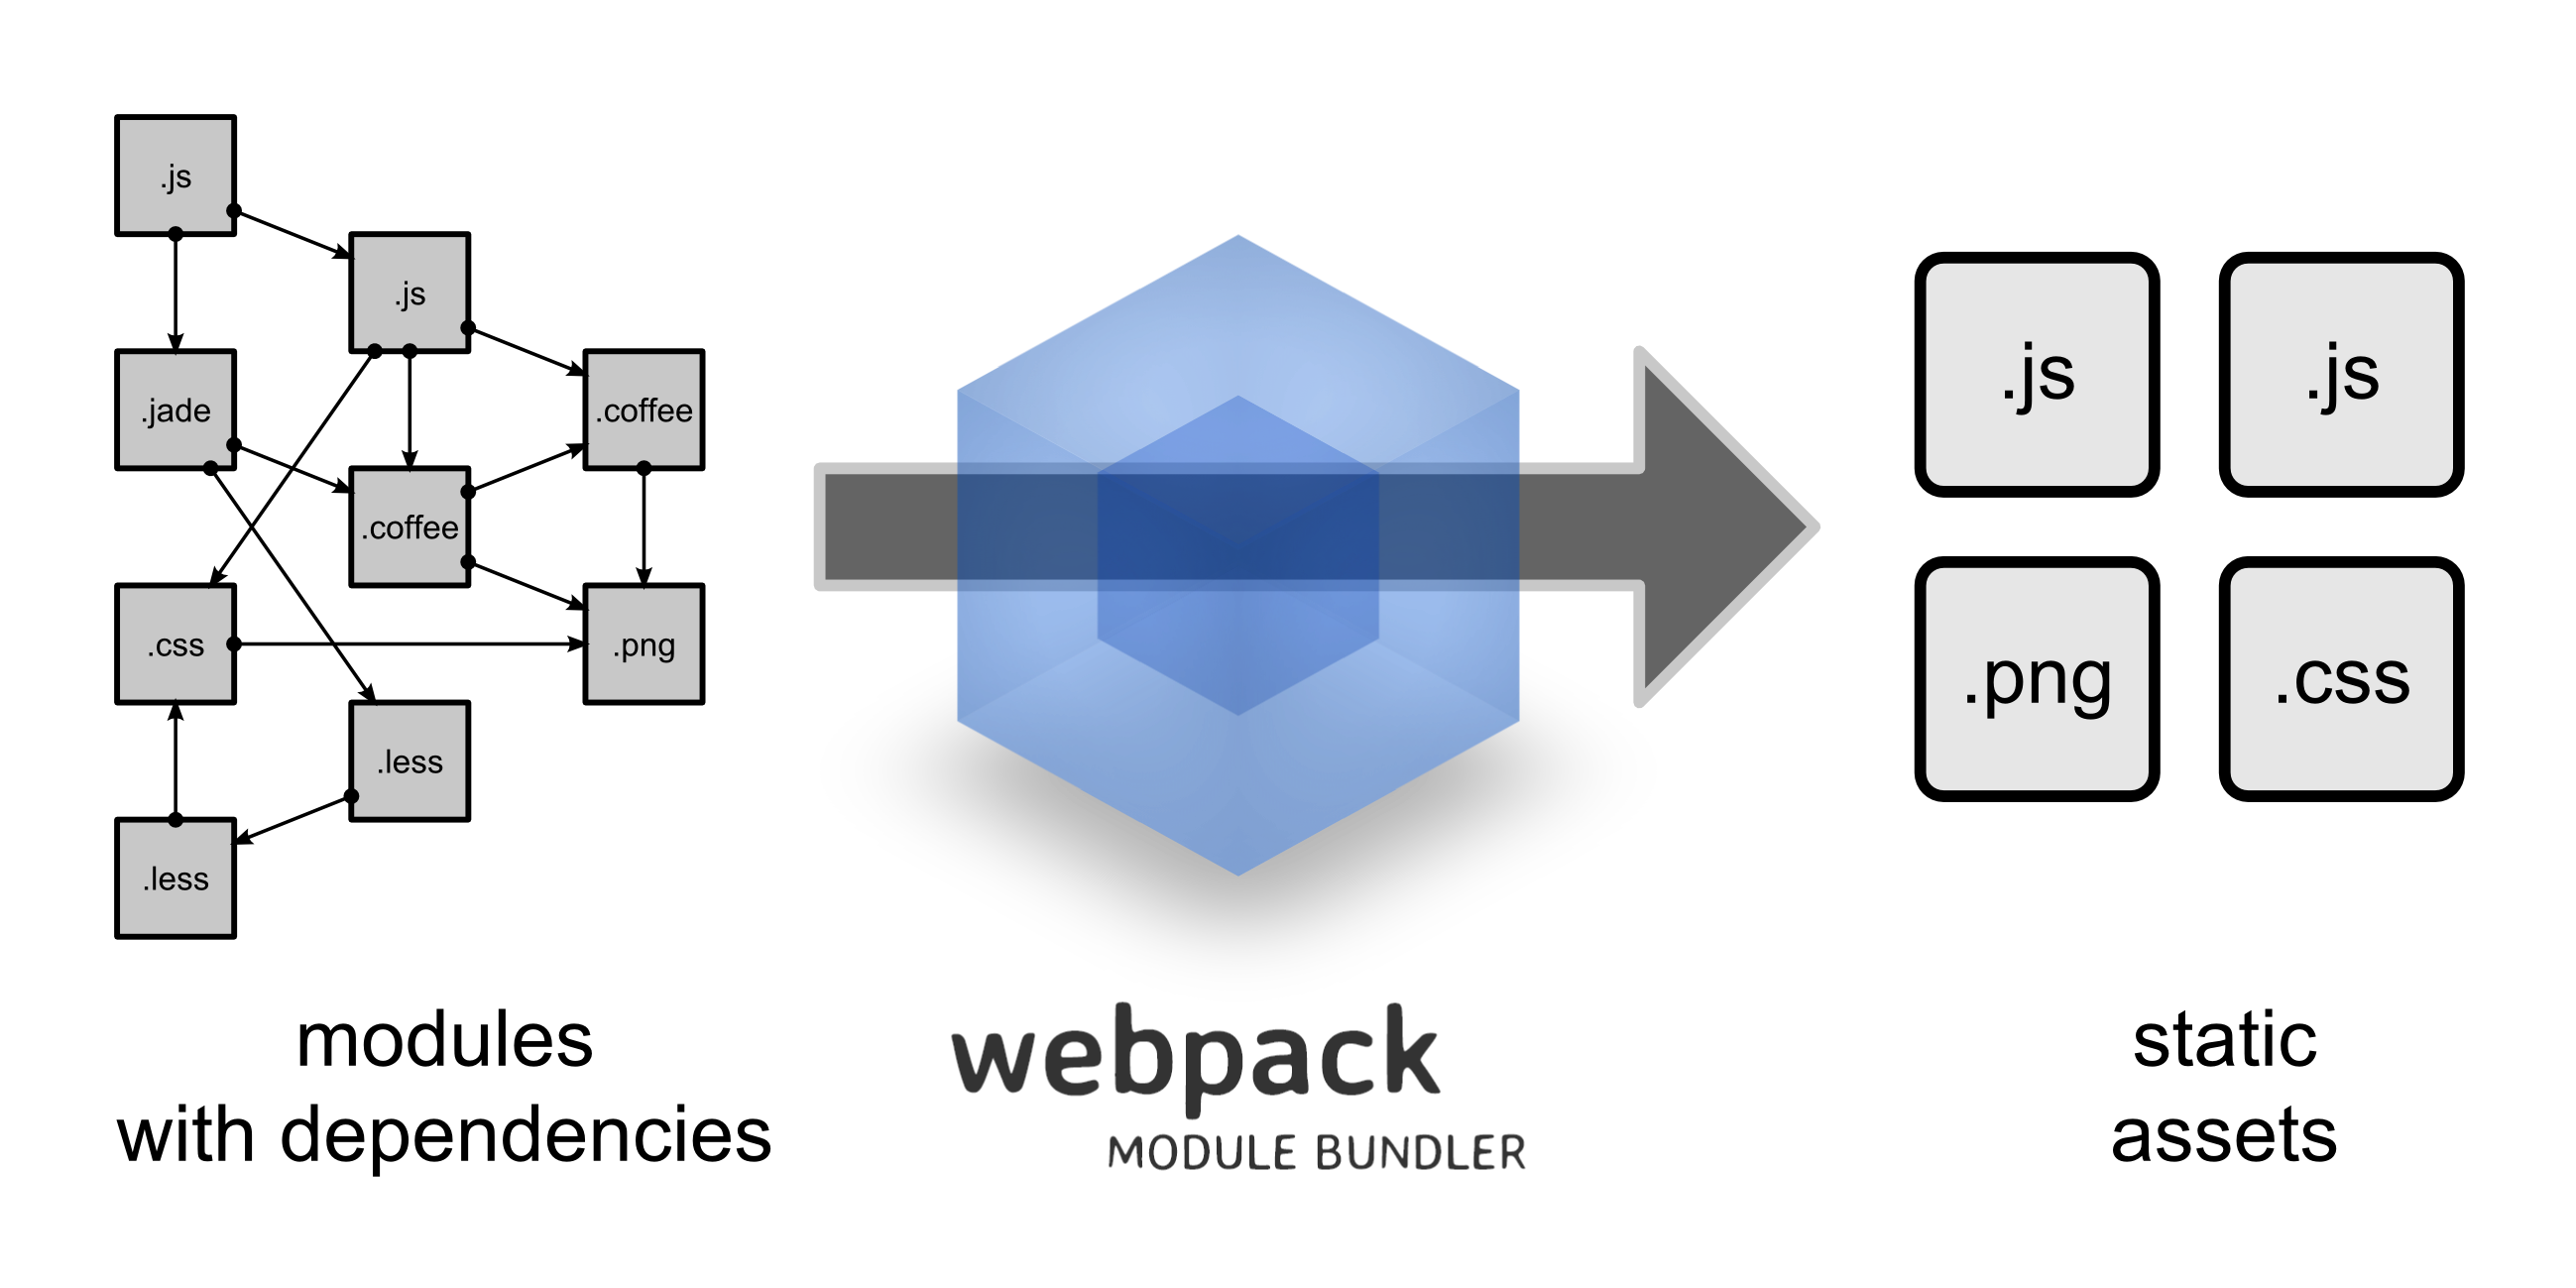
\includegraphics[width=0.8\textwidth]{images/cap4/webpack.eps}
\caption{Imagen descriptiva de Webpack}
\label{fig:Imagen descriptiva de Webpack}
\end{center}
\end{figure}


Como resultado final se obtiene una serie de paquetes que contienen todas las dependencias resueltas.

%++++++++++++++++++++++++++++++++++++++++++++++++++++++++++++++++++++++++++++++
\section{Tecnología para la documentación}
\label{4:sec4}
Para integrar la documentación en la nueva aplicación web de SIMDE resultaba obvio que esta documentación
estuviera también en formato web. Para esto existían muchas alternativas, desde un conjunto de ficheros
html hasta un pequeño sistema de gestión de contenidos. 

\bigskip
Dado que la documentación es bastante extensa pero que en realidad, no es más que un documento 
que se redactará en una ocasión y se le irán realizando pequeñas ampliaciones y/o correcciones
se optó por una solución diferente, los generadores de contenido estático.

\subsection{Generadores de contenido estático}

Los generadores de contenido estático se encargan -resumido de forma tosca y breve- de generar 
un conjunto de htmls y css a partir de una plantilla y una serie de ficheros fuentes. 

\bigskip
Este tipo de generadores estáticos tienen un gran auge entre los desarrolladores que desean 
mantener un blog -yo mismo por ejemplo, tengo uno hecho en Hugo-. 

\bigskip 
Existen múltiples ventajas de utilizar este tipo de tecnologías, pero sin duda para mi la más
importante, es que se alimentan de un formato como es el markdown. El cual es muy intuitivo de 
usar y tiene soporte más allá de este tipo de tecnologías. 

\subsection{Hexo}

Hexo es un generador de contenido estático basado en NodeJS. No posee demasiadas diferencias destacables
sobre el resto de alternativas, y ha sido escogido para este proyecto por dos motivos principales:

\begin{enumerate}

\item No me resulta desconocido, ya que lo he utilizado durante cierto tiempo.

\item Al estar basado en Javascript todo queda enfocado hacia un mismo ecosistema dando una sensación
más uniforme respecto al resto del proyecto.

\end{enumerate}
